\chapter{Implementacija i korisničko sučelje}
		
		
		\section{Korištene tehnologije i alati}
		
			Komunikacija u timu ostvarena je kombinacijom \textbf{Atlassian Jira}, \textbf{Atlassian Confluence} i \textbf{WhatsApp}. Za upravljanje kodom korišten je sustav \textbf{Git} i web platforma \textbf{GitHub} za pregled udaljenog repozitorija i bolje snalaženje u projektu.
			Kao razvojno okruženje korišteni su \textbf{Microsoft Visual Studio Code} i \textbf{JetBrains PyCharm}. Microsoft Visual Studio Code je code editor koji podržava različite programske jezike, uključujući C++, Python i mnoge druge. Ovo okruženje dolazi s alatima za uređivanje koda, debugiranje i upravljanje datotekama i kontejnerima.
			S druge strane, \textbf{JetBrains PyCharm} je posebno usmjeren na podršku Python razvoju. Ovaj IDE pruža bogat skup značajki, uključujući pametno završavanje koda, analizu koda, integrirano upravljanje verzijama, i podršku za virtualno okruženje. Korištenjem ova dva razvojna okruženja, tim je imao pristup snažnim alatima za učinkovit i produktivan razvoj softvera.
			Aplikacija je napisana koristeći radni okvir \textbf{FastAPI} koji se koristi za izradu API-ja u pythonu. Za izradu \textit{frontenda} koristili smo \textbf{React} i \textbf{TypeScript}. Prednost \textbf{TypeScripta} nad običnim \textbf{JavaScriptom} je u njegovoj mogućnosti definiranja tipa varijabli i posljedično tome, lakšem rukovanju greškama i boljom kontrolom varijabli.
			Za izradu kontejnera je korišten \textbf{Docker}, a sve je stavljeno na poslužitelja u oblaku na \textbf{Microsoft Azure}.
			
			
			
			\eject 
		
	
		\section{Ispitivanje programskog rješenja}
			
			
			\subsection{Ispitivanje komponenti}
			
			\subsubsection{Ispitni slučaj 1: Registracija korisnika}
				\begin{packed_item}
					
					\item Testira se rad funkcije \texttt{register()} iz \texttt{auth\_services.py}.
					\item Mock-anje autentikacije i spremanja korisnika u bazu.
					\item Očekivani response: HTTP 201 CREATED.
				\end{packed_item}
				
			\subsubsection{Ispitni slučaj 2: Neispravna registracija korisnika}
				\begin{packed_item}
					\item Testira se funkcija register() s pogrešnim podatkom "role", daje mu se nepostojeća uloga.
					\item Očekivani response: ValidationError
				\end{packed_item}
			
			\subsubsection{Ispitni slučaj 3: Ispravno kreiranje problema}
				\begin{packed_item}
					\item Testira se funkcija \texttt{create\_problem()}
					\item Mock-anje form date za popunjavanje forme za kreiranje problema.
					\item Očekivani response: HTTP 201 CREATED
				\end{packed_item}
			
			\subsubsection{Ispitni slučaj 4: Neispravno kreiranje problema}
				\begin{packed_item}
					\item Form data popunjena neispravnim podacima.
					\item očekivani response: HTTP 422
			 	\end{packed_item}	
			 	
			\subsubsection{Ispitni slučaj 5: Ispravno kreiranje natjecanja}
				\begin{packed_item}
					\item Mock- anje form date za kreiranje natjecanja
					\item Očekivani response: HTTP 201 CREATED
				\end{packed_item}
				
			\subsubsection{Ispitni slučaj 6: Neispravno kreiranje natjecanja}
				\begin{packed_item}
					\item Mock form date s nedovoljno podataka
					\item Očekivani response: HTTP 422
				\end{packed_item}
				
			\eject
			
			
			\subsection{Ispitivanje sustava}
			
			\subsubsection{Ispitni slučaj 1: Ispravna prijava u sustav}
			
			
			\noindent {\textbf{Ulaz:}}
			\begin{packed_enum}
				
				\item  Otvaranje početne stranice u web pregledniku.
				\item  Pritisak na gumb \textbf{Login} u gornjem desnom kutu.
				\item  Ispravno ispunjavanje forme za prijavu.
				\item  Pritisak na gumb \textbf{Submit}. 
				
			\end{packed_enum}
			
			\noindent {\textbf{Očekivani rezultat:}}
			\begin{packed_enum}
				
				\item  Prikaz početne stranice korisnika. 
				
			\end{packed_enum}
			
			\noindent \textbf{Rezultat:} Očekivani rezultat [1.] je zadovoljen jer je korisnik ispravno unio podatke. \textbf{Aplikacija je prošla test.}
			
			\begin{figure}[H]
				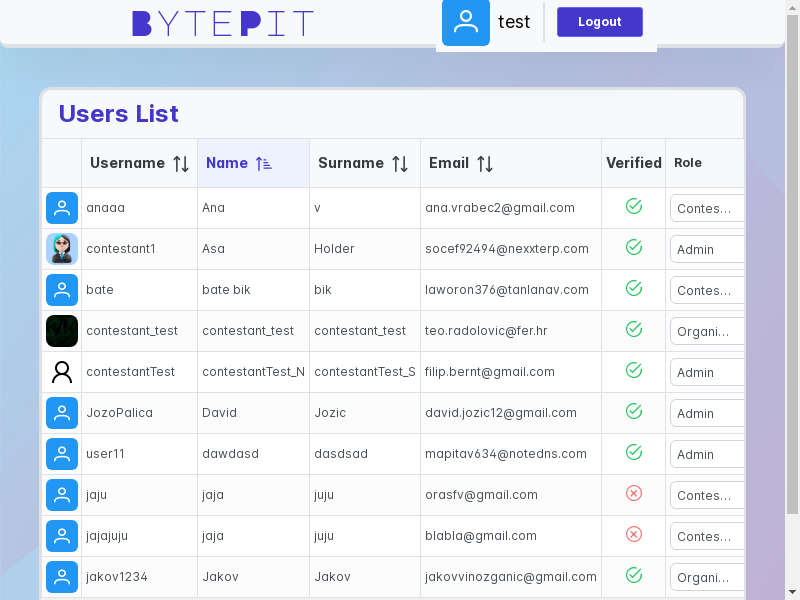
\includegraphics[scale=0.50]{slike/screenshot_test_result.PNG}
				\centering
				\caption{Uspješna prijava}
				\label{fig:sucess_login}
			\end{figure}
			
			\eject
			
			\subsubsection{Ispitni slučaj 2: Neispravna prijava u sustav}
			
			
			\noindent {\textbf{Ulaz:}}
			\begin{packed_enum}
				
				\item  Otvaranje početne stranice u web pregledniku.
				\item  Pritisak na gumb \textbf{Login} u gornjem desnom kutu.
				\item  Ispunjavanje forme za prijavu.
				\item  Pritisak na gumb \textbf{Submit}. 
				
			\end{packed_enum}
			
			\noindent {\textbf{Očekivani rezultat:}}
			\begin{packed_enum}
				
				\item  Prikaz oblačića sa tekstom koji govori da je pogrešno unesena zaporka ili e-pošta/korisničko ime. 
				
			\end{packed_enum}
			
			\noindent \textbf{Rezultat:} Očekivani rezultat [1.] je zadovoljen jer je korisnik unio pogrešnu zaporku. \textbf{Aplikacija je prošla test.}
			
			\begin{figure}[H]
				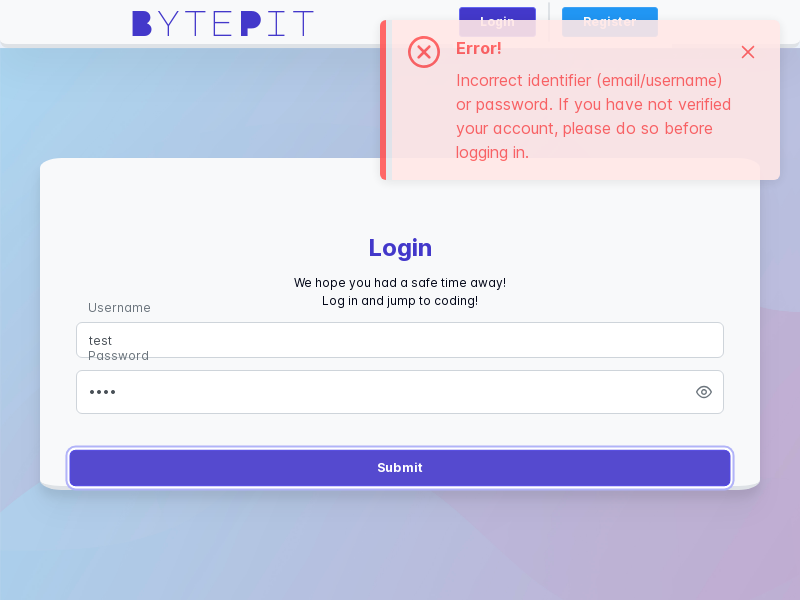
\includegraphics[scale=0.50]{slike/failed_login.PNG}
				\centering
				\caption{Neuspješna prijava}
				\label{fig:failed_login}
			\end{figure}
			
			\eject
			
			\subsubsection{Ispitni slučaj 3: Ispravna registracija novog korisnika}
			
			
			\noindent {\textbf{Ulaz:}}
			\begin{packed_enum}
				
				\item  Otvaranje početne stranice u web pregledniku.
				\item  Pritisak na gumb \textbf{Register} u gornjem desnom kutu.
				\item  Ispunjavanje forme za registraciju.
				\item  Pritisak na gumb \textbf{Submit}. 
				
			\end{packed_enum}
			
			\noindent {\textbf{Očekivani rezultat:}}
			\begin{packed_enum}
				
				\item  Uspješno slanje forme za kreaciju novog korisnika.
				\item  Dobitak e-pošte za verifikaciju novog računa.
				
			\end{packed_enum}
			
			\noindent \textbf{Rezultat:} Očekivani rezultati [1., 2.] su zadovoljeni jer je korisnik ispravno unio podatke koji su traženi. \textbf{Aplikacija je prošla test.}
			
			\begin{figure}[H]
				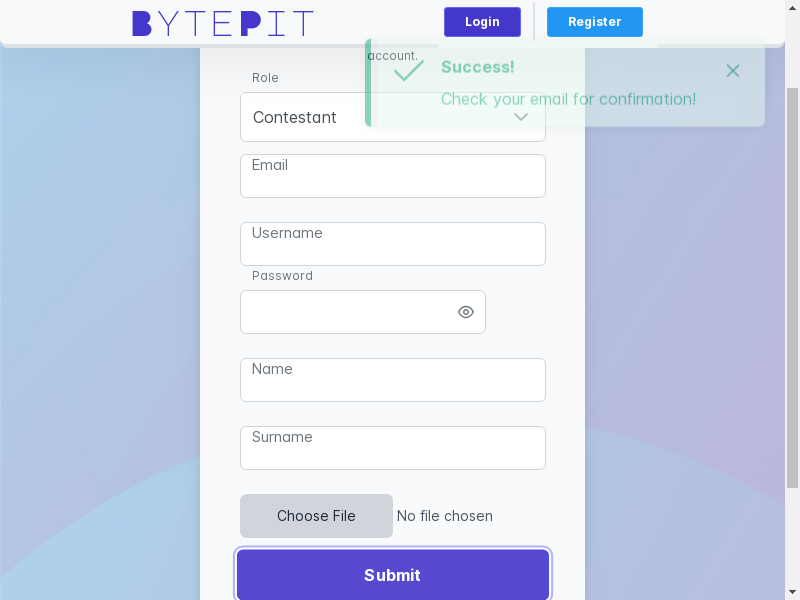
\includegraphics[scale=0.50]{slike/registration_new_user_test_result.PNG}
				\centering
				\caption{Uspješna registracija}
				\label{fig:sucess_register}
			\end{figure}
			
			\eject
			
			\subsubsection{Ispitni slučaj 4: Neispravna registracija novog korisnika}
			
			
			\noindent {\textbf{Ulaz:}}
			\begin{packed_enum}
				
				\item  Otvaranje početne stranice u web pregledniku.
				\item  Pritisak na gumb \textbf{Register} u gornjem desnom kutu.
				\item  Neispravno ispunjavanje forme za registraciju (korištenje e-pošte koja se već nalazi u sustavu).
				\item  Pritisak na gumb \textbf{Submit}. 
				
			\end{packed_enum}
			
			\noindent {\textbf{Očekivani rezultat:}}
			\begin{packed_enum}
				
				\item  Neuspješno slanje forme za kreaciju novog korisnika.
				\item  Prikaz oblačića sa tekstom koji govori da se e-pošta već koristi.
				
			\end{packed_enum}
			
			\noindent \textbf{Rezultat:} Očekivani rezultati [1., 2.] su zadovoljeni jer je korisnik unio e-poštu koja se već koristi. \textbf{Aplikacija je prošla test.}
			
			\begin{figure}[H]
				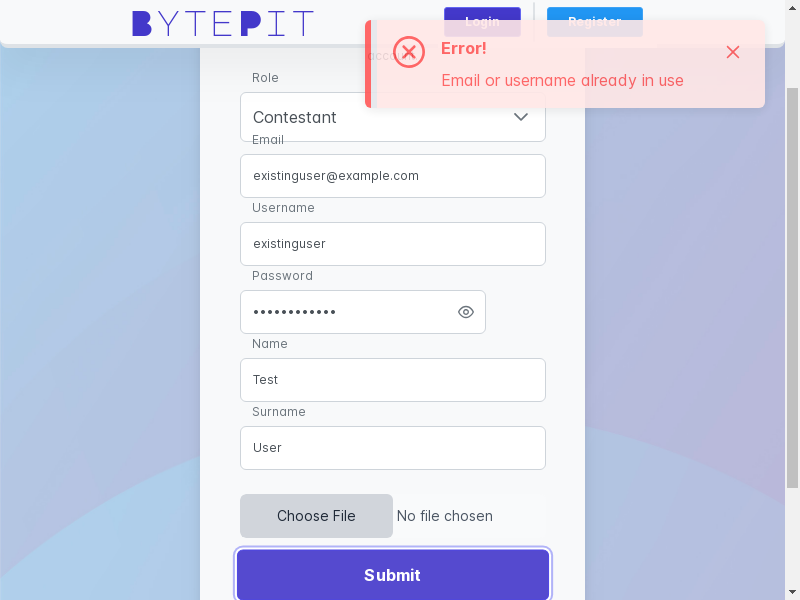
\includegraphics[scale=0.50]{slike/registration_already_exists_test_result.PNG}
				\centering
				\caption{Uspješna registracija}
				\label{fig:failed_register}
			\end{figure}
			
			\eject
			
			\subsubsection{Ispitni slučaj 5: Uspješna odjava korisnika}
			
			
			\noindent {\textbf{Ulaz:}}
			\begin{packed_enum}
				
				\item  Pritisak na gumb \textbf{Logout} na stranici korisnika.
				
			\end{packed_enum}
			
			\noindent {\textbf{Očekivani rezultat:}}
			\begin{packed_enum}
				
				\item  Prikaz stranice za prijavu u sustav.
				
			\end{packed_enum}
			
			\noindent \textbf{Rezultat:} Očekivani rezultat [1.] je zadovoljen. \textbf{Aplikacija je prošla test.}
			
			\begin{figure}[H]
				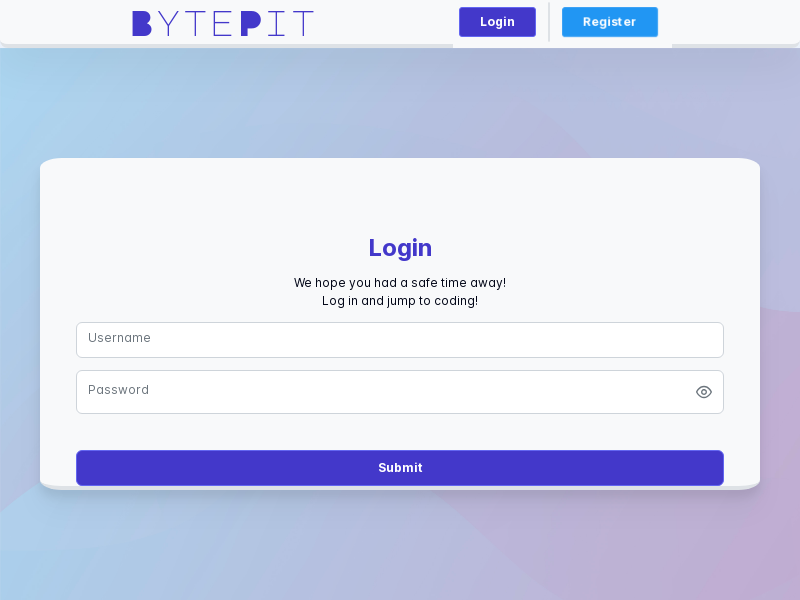
\includegraphics[scale=0.50]{slike/screen_after_logout.PNG}
				\centering
				\caption{Uspješna odjava}
				\label{fig:sucess_logout}
			\end{figure}
			
			
			\eject 
		
		
		\section{Dijagram razmještaja}

			 Dijagrami razmještaja opisuju topologiju sklopovlja i programsku potporu koja se koristi u implementaciji sustava u njegovom radnom okruženju.
			 Na azure app service-u nalaze se API sa evaluatorom rješenja, poslužitelj baze podataka (azure sql database) te third party servis za kompajliranje koda.
			 Klijenti koriste web preglednik za pristup web aplikaciji. Sustav je baziran na kombiniranoj RPC i REST API arhitekturi, a komunikacija između klijenta i poslužitelja odvija se preko HTTP veze.

			 
			
			\begin{figure}[H]
				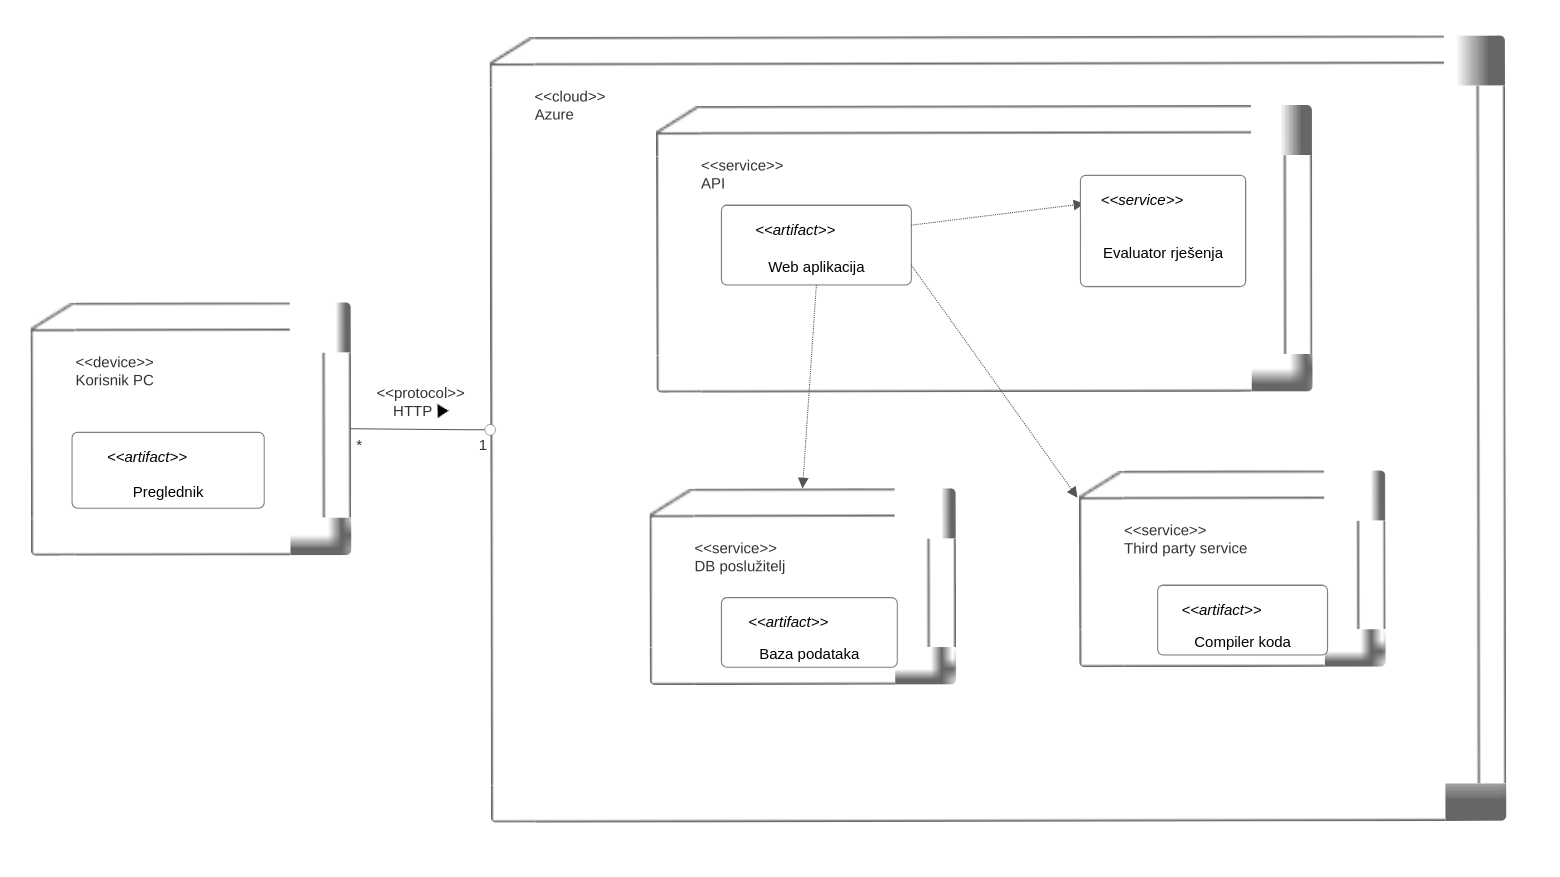
\includegraphics[width=\linewidth]{slike/dijagram_razmjestaja.png} 
				\centering
				\caption{Dijagram razmještaja}
				\label{fig:razmjestaj}
			\end{figure}
			\eject 
		
		\section{Upute za puštanje u pogon}
		
			\textbf{Pokretanje backend-a i baze podataka}\\
			
				\noindent Potrebno je klonirati sve projekte iz GitHub organizacije \href{https://github.com/ProgiRade}{ProgiRade}. Na Windowsu je potrebno preuzeti i instalirati aplikaciju \href{https://www.docker.com/products/docker-desktop/}{Docker Desktop} uz pomoć koje se pokreću containeri za backend i bazu podataka. Nakon preuzimanja aplikacije potrebno je u terminalu navigirati do direktorija \textit{bytepit-root} unutar kojeg se nalazi docker-compose datoteka koja sadrži informacije za pokretanje. Pri prvom pokretanju potrebno je nekoliko minuta za podizanje.\\
				Unutar terminala koristimo naredbu: \textbf{docker-compose up --build}
				\begin{figure}[H]
					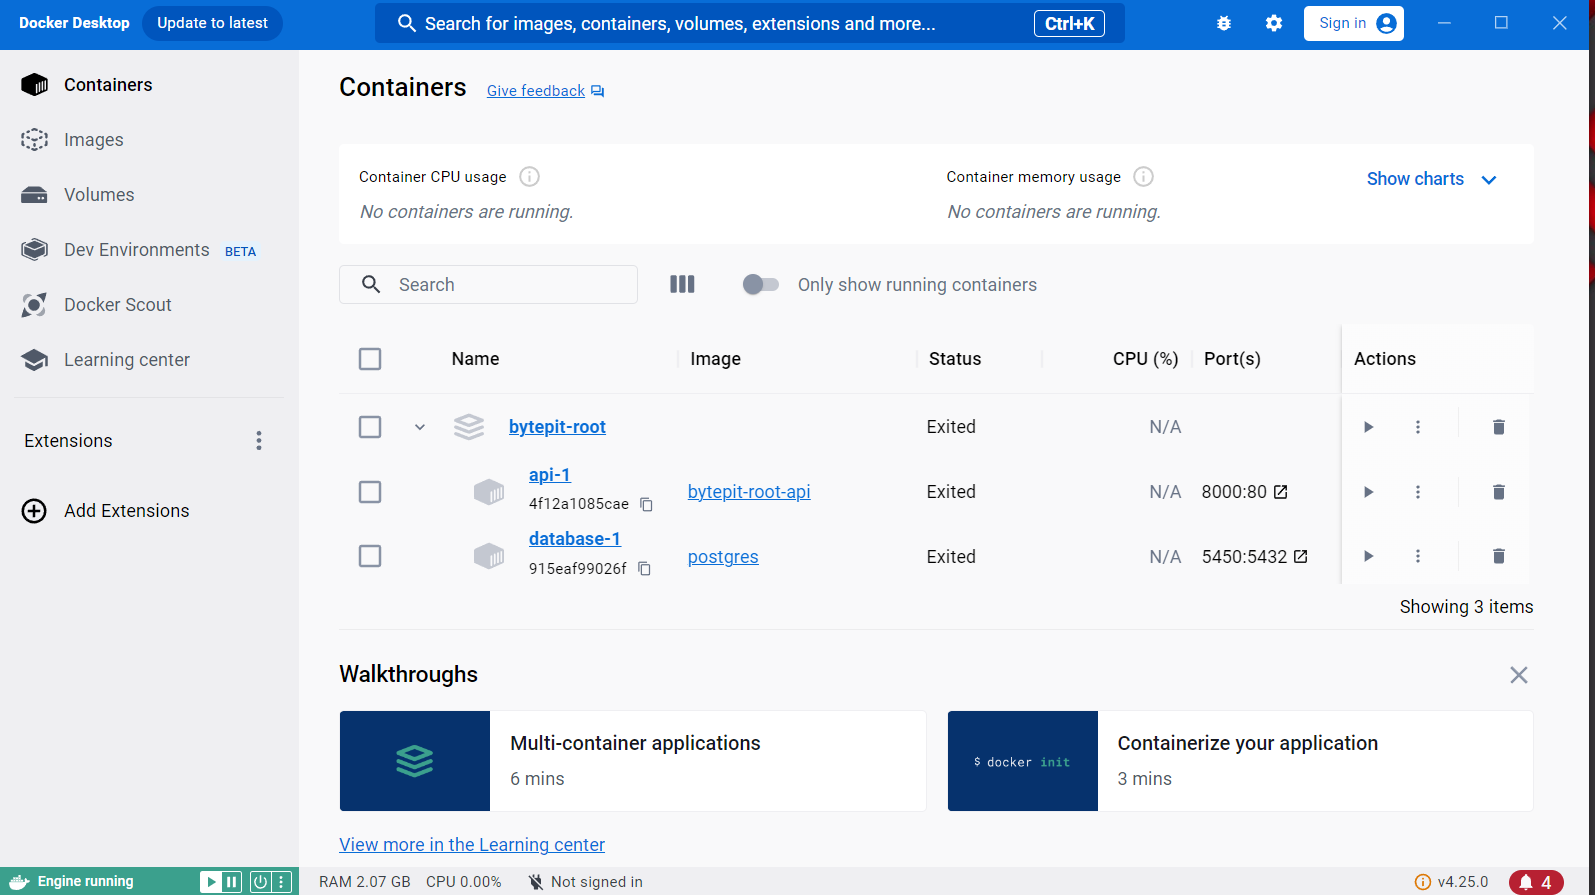
\includegraphics[scale=0.45]{slike/docker_desktop.PNG} 
					\centering
					\caption{Aplikacija Docker Desktop sa kreiranim containerima}
					\label{fig:docker_desktop}
				\end{figure}
				\noindent Pri prvom pokretanju unutar baze neće biti kreirane potrebne tablice, ali ih možemo kreirati uz pomoć datoteke \textbf{ddl.sql} koja se nalazi unutar direktorija \textit{bytepit-root}. Unutar aplikacije Docker Desktop možemo kliknuti na opcije od baze (tri uspravne točkice ispod zaglavlja Actions), te odabrati opciju \textbf{Open in terminal} uz pomoć koje možemo upisati naredbe za kreaciju tablica unutar baze. Unutar terminala odabiremo opciju \textbf{Exec} te u njoj napišemo naredbu: \textbf{psql -U postgres -d db}\\
				\noindent Na Linuxu je procedura slična, može se iz terminala direktno pristupiti bazi podataka uz pomoć naredbe: \textbf{psql -h localhost -p 5450 -U postgres -d db}\\
				\eject
				\noindent Tada možemo pisati naredbe za našu bazu u SQL-u unutar terminala. Sljedeća naredba koju unosimo je cijela \textbf{ddl.sql} datoteka uz pomoć koje se kreiraju tablice. Nakon toga su backend i baza podataka uspješno postavljeni i spremni za korištenje. Kao provjeru za ispravno kreiranje tablica možemo napisati query poput ovoga:\\
				\textbf{SELECT * FROM problems;}, u slučaju ispravnog postavljanja ispisuje se tablica \textit{problems}.\\
				\begin{figure}[H]
					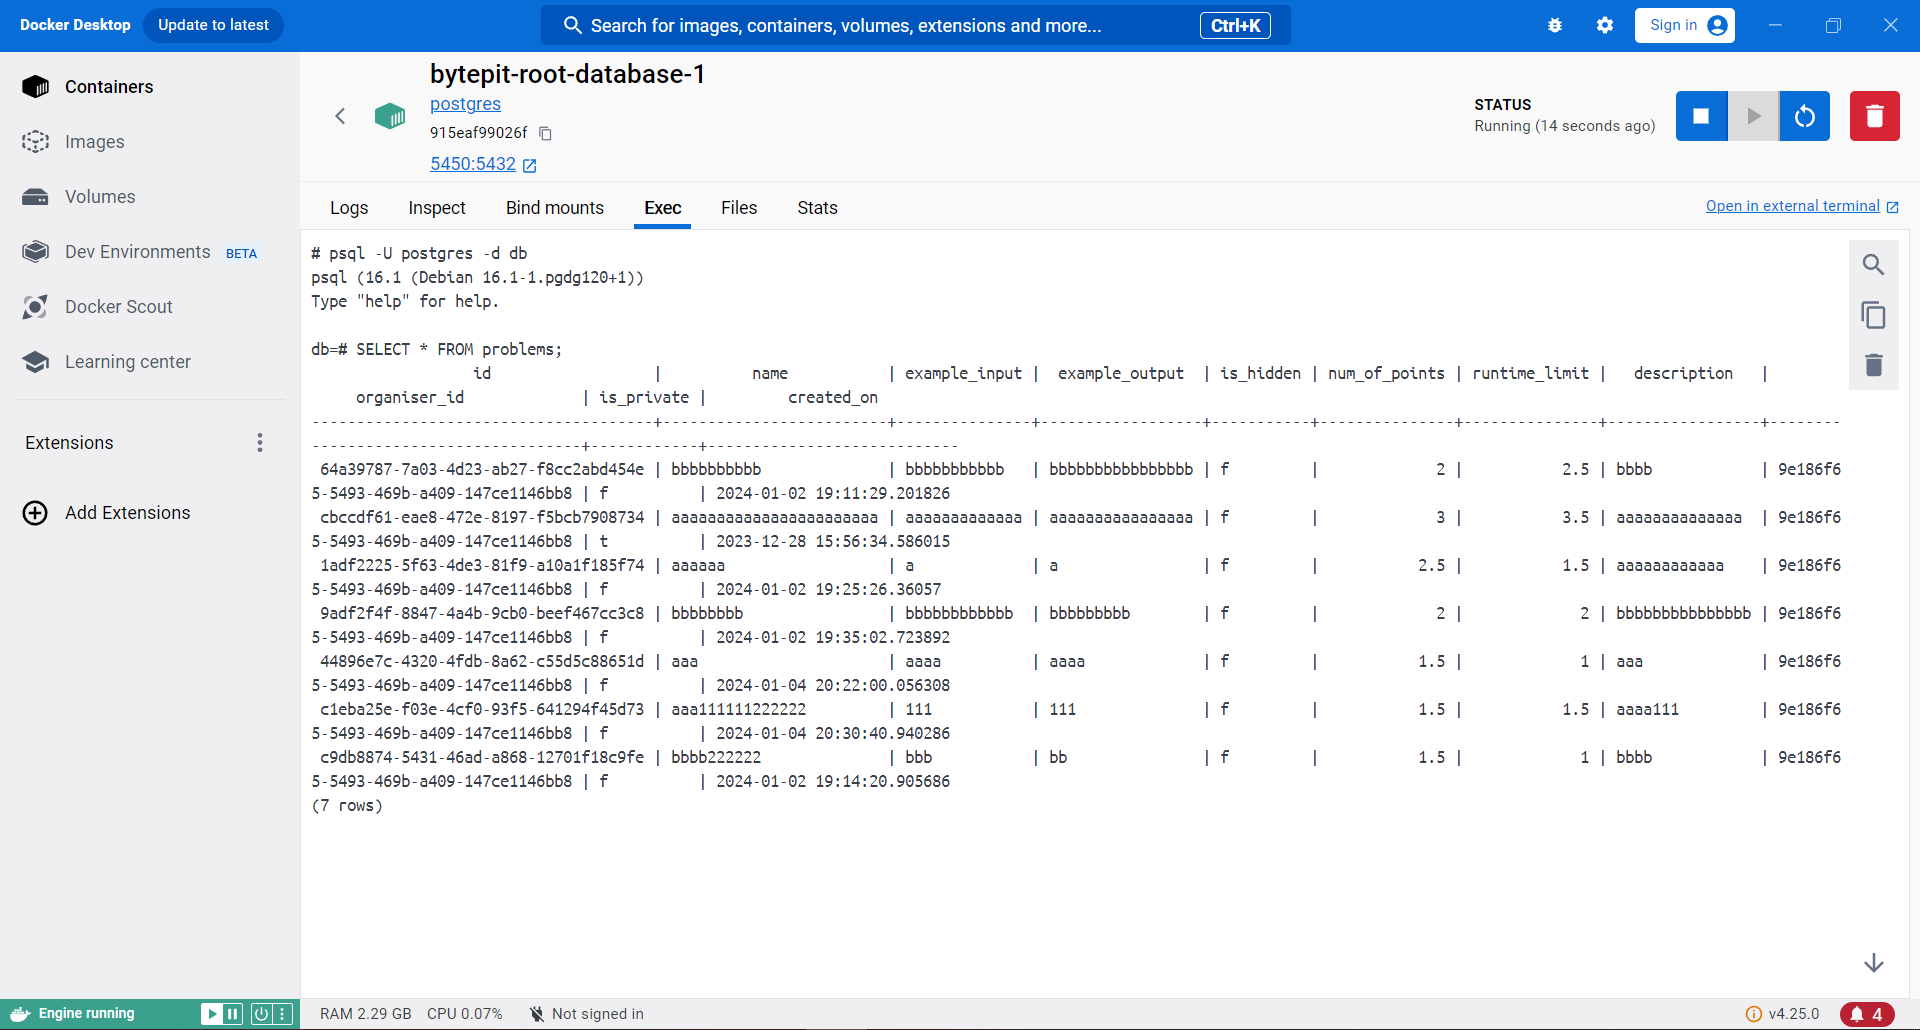
\includegraphics[scale=0.4]{slike/postgres.PNG} 
					\centering
					\caption{Ispravno ispunjena baza i provjera}
					\label{fig:docker_desktop_postgres}
				\end{figure}
				\noindent Za zaustavljanje Docker container-a koristimo naredbu: \textbf{docker-compose down}\\
				
			\eject
			
			\noindent\textbf{Pokretanje frontend-a}\\
			
			\noindent Unutar terminala se navigiramo do direktorija \textit{bytepit-ui} te pokrećemo naredbu: \textbf{npm install}\\
			Pomoću te naredbe se pokreće instalacija Vite-a i ostalih dependencyja koji su potrebni za pokretanje frontenda. Za instalaciju je potrebno nekoliko minuta.\\
			\noindent Nakon instalacije pokrećemo naredbu: \textbf{npm run dev} koja pokreće frontend.
			\begin{figure}[H]
				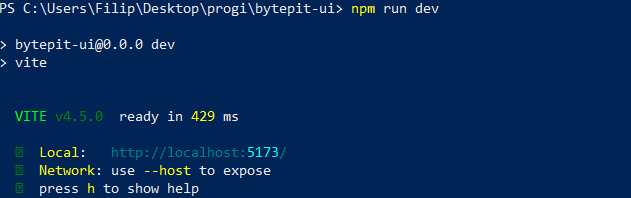
\includegraphics[scale=0.9]{slike/vite.PNG} 
				\centering
				\caption{Terminal nakon uspješno izvedene funkcije za pokretanje}
				\label{fig:vite}
			\end{figure}
			\noindent Tada možemo otvoriti web-preglednik i upisati \textbf{http://localhost:5173/} i početi koristiti aplikaciju.\\
			\begin{figure}[H]
				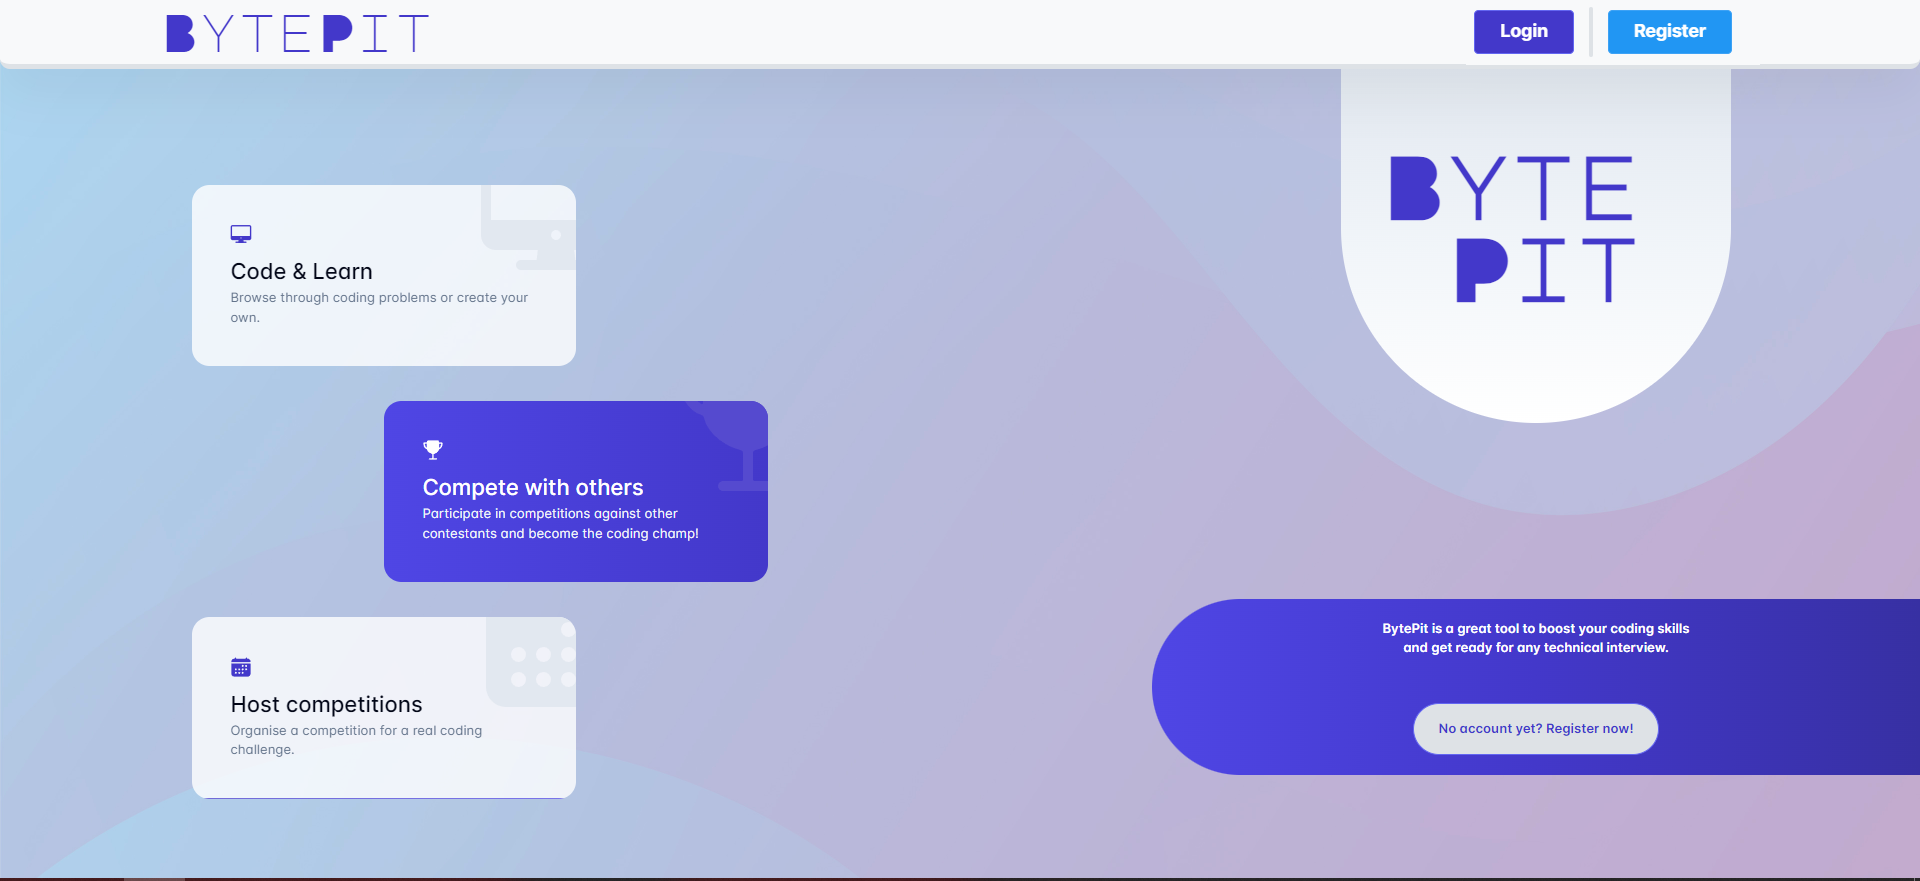
\includegraphics[scale=0.4]{slike/bytepit.PNG} 
				\centering
				\caption{Pokrenuta aplikacija}
				\label{fig:bytepit}
			\end{figure}
			